A participação cidadã e a colaboração em governos eletrônicos (e-Gov) têm se tornado cada vez mais relevantes na sociedade contemporânea. Com o avanço da tecnologia e a disseminação das redes sociais, surgiram novas formas de engajamento e interação entre cidadãos e governos. Nesse contexto, o aplicativo Colab.re posiciona como uma plataforma inovadora que combina elementos de redes sociais com a participação cidadã em questões relacionadas à gestão pública. Neste capítulo, exploraremos o Colab.re sob a perspectiva das redes sociais, e-Gov e Gov techs e vigilância participativa, analisando suas funcionalidades, impactos sociais, desafios e limitações.


\section*{História e Desenvolvimento}
O Colab.re foi lançado em 2013 como uma iniciativa pioneira no campo da participação cidadã digital. A plataforma foi desenvolvida pelos sócios Paulo Pandolfi e Gustavo Maia, que, inspirados por suas experiências em marketing político, perceberam a necessidade de uma ferramenta que permitisse uma maior interação entre cidadãos e governos \cite{2023_Colab_PAGE}.

O objetivo do Colab.re é permitir que os usuários compartilhem ideias, façam sugestões, denunciem problemas e participem ativamente na construção de políticas públicas. Funcionando como uma rede social, os cidadãos podem postar fotos de problemas da cidade e solicitar uma solução. As prefeituras, por sua vez, acessam essas reclamações e têm uma solução de tecnologia em nuvem para dar andamento às solicitações \cite{2023_Colab_PAGE}.

Desde o seu lançamento, o Colab.re tem conquistado espaço em diversas cidades, tornando-se uma ferramenta de referência no campo da democracia digital. A plataforma foi eleita “o melhor app urbano do mundo” pela NewCities Foundation e hoje conta com 200 mil cadastros e contratos com diversas cidades, incluindo Recife, Ipojuca, Niterói, Mesquita, Maceió, Aracaju, Cruz Alta, Santo André e Juiz de Fora \cite{2023_Colab_PAGE}.

Além disso, desde 2016, o Colab.re também oferece uma ferramenta para que as prefeituras abram consultas sobre questões da cidade, auxiliando na tomada de decisões e na coleta de dados. Essa ferramenta tem vários formatos e gera muitos dados que ajudam a fazer uma gestão melhor com a participação do cidadão \cite{2023_Colab_PAGE}.

A história do Colab.re é marcada por desafios e inovações. Quando foi lançado, o aplicativo não tinha nenhuma prefeitura cadastrada. As necessidades dos cidadãos eram coletadas pela empresa e enviadas para a administração pública pelos canais de atendimento tradicionais, como site e email. No entanto, mesmo sem prefeituras cadastradas, o sistema foi reconhecido internacionalmente pela NewCities Foundation como "o melhor app urbano do mundo" \cite{2023_Colab_PAGE}.

A primeira prefeitura a adotar oficialmente o Colab.re foi Curitiba, seguida por outras 50 no mesmo ano. Esse crescimento rápido trouxe desafios, pois a empresa precisava atender melhor e evoluir, mas ainda não tinha receita. No entanto, um contrato com a organização social Comunitas, no começo de 2015, para atender as cidades de Santos e Campinas, em São Paulo, e Pelotas, no Rio Grande do Sul, injetou dinheiro na empresa e deu ânimo aos empreendedores \cite{2023_Colab_PAGE}.

Desde a sua fundação, o Colab.re tem buscado desenvolver soluções tecnológicas que possam contribuir para a construção de uma gestão pública mais eficiente, transparente e participativa. Atualmente, a plataforma está presente em mais de 130 cidades, em 2 países, e conta com cerca de 900 mil usuários cadastrados \cite{2023_Colab_PAGE}.

Hoje, a plataforma tem 200 mil cadastros e contratos com diversas cidades, incluindo Recife, Ipojuca, Niterói, Mesquita, Maceió, Aracaju, Cruz Alta, Santo André e Juiz de Fora. O valor dos contratos varia de 38 mil a 500 mil reais por ano, calculado com base na população da cidade e na quantidade de módulos contratados.

\section*{Funcionalidades}

\begin{figure}[!htb]
	\caption{Tela inicial do app Colab.re}
	\label{fig:colab_app}
	\centering
	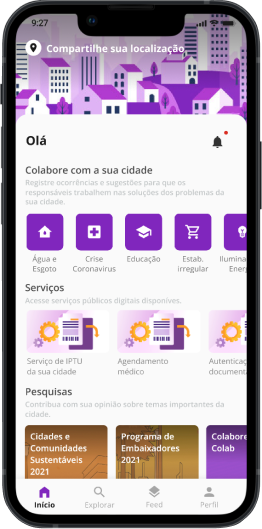
\includegraphics[scale=0.5]{colab_app.png}
\end{figure}

O Colab.re é uma plataforma digital que promove a vigilância participativa, a democracia digital e o governo eletrônico (e-gov) por meio de uma série de funcionalidades interativas. A plataforma se destaca por permitir que os cidadãos desempenhem um papel ativo na gestão pública, contribuindo com ideias, sugestões e denúncias, e participando de consultas públicas.

A funcionalidade de publicação de ideias e sugestões permite que os usuários compartilhem suas ideias sobre questões de interesse público, abrangendo uma variedade de temas, desde melhorias na infraestrutura urbana até propostas de políticas sociais. Essa funcionalidade promove a democracia digital, permitindo que os cidadãos participem ativamente na formulação de políticas públicas.

A funcionalidade de denúncia de problemas permite que os usuários denunciem problemas como buracos nas vias, iluminação pública deficiente, entre outros. Essas denúncias são georreferenciadas, facilitando a identificação e resolução dos problemas pelas autoridades competentes. Isso contribui para a vigilância participativa, pois permite que os cidadãos monitorem a qualidade dos serviços públicos e infraestruturas em suas comunidades.

O Colab.re também possui uma forte componente social. Os usuários podem seguir outros usuários, serem seguidos, curtir e comentar as publicações. Isso promove a formação de uma rede social dentro do Colab.re, ampliando as possibilidades de engajamento e diálogo entre os participantes.

Os usuários também podem acompanhar o andamento das demandas e propostas que foram apresentadas. Isso permite que eles estejam cientes das ações tomadas pelo governo em resposta às suas contribuições, promovendo a transparência e a responsabilidade no governo eletrônico.

Além disso, o Colab.re introduziu recentemente novas funcionalidades, como micro consultas, reportar comentários e priorização de comentários. As micro consultas permitem que os usuários respondam perguntas rápidas do tipo sim/não diretamente na notificação push, trazendo mais dinamismo e velocidade para a gestão do relacionamento entre o cidadão e a cidade. A funcionalidade de reportar comentários permite que os usuários do Colab.re reportem comentários uns dos outros, mantendo a qualidade e a relevância das discussões na plataforma. A priorização de comentários, também conhecida como up/down vote, permite que os usuários indiquem o quão relevante um comentário é por meio de votos, destacando as contribuições mais valiosas.

A funcionalidade de consultas públicas é uma parte essencial do Colab.re, permitindo que os governos interajam diretamente com os cidadãos e obtenham feedback sobre várias questões. As consultas podem ser personalizadas para se adaptarem à realidade de cada território, e os gestores públicos podem criar seus próprios processos. Além disso, é possível configurar as consultas para permitir respostas anônimas. Essa funcionalidade promove a democracia digital e o governo eletrônico, permitindo que os cidadãos participem diretamente na tomada de decisões do governo.

A gamificação é um aspecto central do Colab.re, usada para aumentar o engajamento dos cidadãos e incentivá-los a participar ativamente na melhoria de suas cidades. A gamificação envolve o uso de elementos de design de jogos em contextos não-jogáveis para motivar a participação, envolvimento e lealdade.

No Colab.re, a gamificação é implementada através da "Jornada do Cidadão", uma trilha com desafios que orientam o cidadão sobre como ele pode colaborar e participar mais para tornar sua cidade melhor. Ao completar esses desafios, os cidadãos recebem recompensas e conquistas, que podem ser compartilhadas com outros usuários. Isso não apenas incentiva a participação contínua, mas também ajuda a disseminar uma cultura de participação dentro da cidade.

A gamificação no Colab.re não se limita apenas a incentivar a participação dos cidadãos. Ela também pode ser usada para conscientizar sobre determinadas causas ou estimular a participação em eventos. Por exemplo, se um hemocentro da cidade precisa de mais doações de sangue, a gestão pública pode criar um desafio no Colab.re para incentivar os cidadãos a doar sangue. Ao fazer isso, os cidadãos podem ganhar conquistas como "doador" ou "zelador do patrimônio público", reforçando a importância de suas contribuições para a cidade.

Em resumo, o Colab.re é uma plataforma que combina elementos de vigilância participativa, democracia digital e governo eletrônico para promover a participação cidadã na gestão pública. Através de suas diversas funcionalidades, o Colab.re busca fortalecer a participação cidadã, criar um ambiente propício para o diálogo entre cidadãos e governos, e promover a transparência e a responsabilidade no governo.

\section*{Gov Techs}
As gov techs são empresas que fornecem soluções tecnológicas para o setor público. Elas desempenham um papel crucial na modernização dos serviços governamentais, melhorando a eficiência, a transparência e a participação cidadã. Os serviços prestados ao governo por empresas de gov tech podem variar amplamente, dependendo das necessidades específicas do governo. Alguns exemplos incluem:

\begin{itemize}
	\item Digitalização de processos burocráticos: Isso pode incluir a criação de sistemas de gerenciamento de documentos, plataformas de pagamento online e sistemas de agendamento de compromissos.
	\item Plataformas de participação cidadã: Estas são plataformas que permitem aos cidadãos participar diretamente na tomada de decisões do governo. Isso pode incluir a votação em questões políticas, a apresentação de propostas de políticas e a participação em discussões públicas.
	\item Soluções de análise de dados: As empresas de gov-tech podem fornecer soluções que ajudam o governo a coletar, analisar e interpretar grandes quantidades de dados. Isso pode ajudar o governo a tomar decisões mais informadas e eficazes.
\end{itemize}

O Colab.re é um exemplo de uma solução de gov tech que se destaca na indústria pelo seu aspecto social. Como uma plataforma de participação cidadã, o Colab.re permite que os cidadãos se envolvam diretamente na tomada de decisões do governo, promovendo a transparência e a responsabilidade. Isso representa uma mudança significativa na forma como o governo interage com os cidadãos, permitindo uma maior inclusão e participação na tomada de decisões.

No entanto, a adoção de soluções de gov tech como o Colab.re não está isenta de desafios. De acordo com um estudo de \citeonline{2021_Liang}, fatores como a competência do provedor, a prontidão organizacional, a pressão externa e a confiança na tecnologia desempenham um papel significativo na adoção de tecnologias de nuvem móvel no governo. Esses fatores podem ser igualmente aplicáveis ao Colab.re e outras soluções de gov tech, e precisam ser considerados cuidadosamente ao implementar essas tecnologias.

Além disso, a tecnologia blockchain está emergindo como uma nova ferramenta potencial para o setor público. \citeonline{2021_Diakiv} identifica dez direções potenciais para o uso de tecnologias blockchain no setor público, incluindo autenticação, rastreabilidade e singularidade. Embora o Colab.re não utilize a tecnologia blockchain, a crescente importância dessa tecnologia no setor público sugere que pode ser uma área para futura exploração ou integração.

Finalmente, a ética na tecnologia é uma consideração importante na adoção de soluções de gov tech. \citeonline{2022_Grellette} sugere a realização de auditorias de confiança como uma maneira de melhorar a prática da ética na tecnologia. Isso poderia ser relevante para o Colab.re e outras soluções de gov tech, à medida que buscam ganhar e manter a confiança do público.

\section*{Interfaces para problemas urbanos}
Devido a adoção em massa de aplicativos e a alta disponibilidade da internet, softwares sociais e de vigilância participativa tem se tornado interfaces para problemas urbanos. Essas interfaces têm desempenhado um papel crucial na resolução de questões relacionadas às cidades. Vários estudos de caso têm evidenciado a eficácia dessa ferramenta em abordar desafios urbanos e promover a participação cidadã.

Barros e Rodrigues (2021) avaliou o Colab.re juntamente com outras duas iniciativas de democracia digital, Mudamos e Panela de Pressão. A avaliação considerou diferentes aspectos, como recursos tecnológicos, modos de participação online, atores envolvidos, objetivos políticos das iniciativas e captação de recursos. Os resultados destacaram a importância da estrutura organizacional na compreensão do desenvolvimento bem-sucedido de iniciativas de democracia digital.

Silva e Policarpo (2014) analisou o Colab.re como uma ferramenta de colaboração e mobilidade urbana. Esse estudo ressaltou a relevância do Colab.re como uma plataforma que permite aos cidadãos participarem ativamente da melhoria de suas cidades, fornecendo um canal direto de feedback às autoridades municipais sobre problemas urbanos.

Em Belém, Brasil, o Colab.re foi utilizado como uma ferramenta para coletar dados sobre a percepção dos cidadãos em relação à qualidade dos serviços públicos, conforme apresentado no estudo de caso de Braga et al. (2021). Os resultados indicaram que o Colab.re pode ser uma ferramenta eficaz para coletar o feedback dos cidadãos e, assim, melhorar a prestação dos serviços públicos.

Por fim, o estudo de caso de Gonçalves et al. (2016) explorou o uso do Colab.re como uma ferramenta para promover a participação cidadã na gestão de resíduos sólidos em uma cidade brasileira. Esse estudo concluiu que o Colab.re pode ser uma ferramenta eficaz para envolver os cidadãos nesse processo e, consequentemente, promover a sustentabilidade urbana.

Esses estudos de caso fornecem evidências concretas de como o Colab.re tem sido uma interface valiosa na resolução de problemas urbanos. Sua capacidade de promover a participação cidadã, coletar feedback dos cidadãos e melhorar a prestação de serviços públicos o torna uma ferramenta relevante para impulsionar mudanças positivas nas cidades. Através do Colab.re e de outras interfaces similares, é possível fortalecer a colaboração entre os cidadãos, autoridades municipais e outros atores envolvidos na busca por soluções inovadoras e sustentáveis para os desafios urbanos.

\section*{Participação cidadã na pandemia de COVID-19}
A pandemia de COVID-19 apresentou desafios sem precedentes para a participação cidadã e o engajamento social. Em resposta a esses desafios, plataformas digitais emergiram como ferramentas vitais para facilitar a participação cidadã na gestão pública, mesmo em meio ao distanciamento social.

\subsection*{Vigilância Participativa}
A vigilância participativa é uma abordagem inovadora que envolve o engajamento ativo da comunidade no processo de coleta, monitoramento e compartilhamento de informações relevantes para identificar e responder a problemas sociais, ambientais e de saúde. 

\begin{citacao}
	"uma forma de inteligência coletiva em que as pessoas se reúnem para monitorar, analisar e agir coletivamente em relação a um problema ou questão compartilhada" \cite[p. 1]{2011_Bryer}.
\end{citacao}

Com os avanços tecnológicos e a disseminação de dispositivos móveis e plataformas digitais, a aplicação de aplicativos móveis para a vigilância participativa tem ganhado destaque. Nesta seção, exploramos o conceito de vigilância participativa, apresentando sua definição e abordando sua relevância no contexto atual.

A vigilância participativa tem sido reconhecida como uma abordagem promissora para a coleta de informações em tempo real, permitindo que a comunidade desempenhe um papel ativo na detecção e monitoramento de problemas sociais, ambientais e de saúde. Tradicionalmente, a vigilância tem sido realizada por meio de sistemas centralizados e conduzida por especialistas em saúde ou autoridades governamentais. No entanto, com a proliferação de dispositivos móveis, o acesso à internet e o surgimento de plataformas colaborativas, os aplicativos móveis têm sido adotados como ferramentas eficazes para engajar os cidadãos na vigilância participativa.

O conceito de vigilância participativa foi formalmente reconhecido pelas Regulamentações Sanitárias Internacionais (RSIs) revisadas em 2005, as quais ampliaram o escopo da vigilância além dos mecanismos tradicionais. Esse reconhecimento proporcionou uma oportunidade para a integração de canais não oficiais e melhorias tecnológicas para agilizar a detecção, o monitoramento e a resposta a problemas de saúde. A vigilância participativa utiliza métodos de crowdsourcing para coletar informações da sociedade e devolver o conhecimento coletivo de volta à comunidade.\cite[1]{2017_Smolinski}

Um estudo de caso relevante que exemplifica a aplicação da vigilância participativa é a iniciativa "Saúde na Copa" durante a Copa do Mundo FIFA de 2014, realizada no Brasil. O projeto utilizou um aplicativo de vigilância participativa chamado Healthy Cup, permitindo que usuários de todo o mundo relatassem suas condições de saúde em tempo real. Ao focar em três síndromes específicas e seis doenças relevantes para aglomerações de pessoas, o aplicativo facilitou a detecção precoce de surtos de doenças agudas ao identificar agregados de sintomas indicativos de doenças infecciosas \cite{2017_LealNeto}.

Além da saúde, a vigilância participativa também tem sido aplicada em outras áreas, proporcionando benefícios semelhantes e promovendo a participação ativa da comunidade. Essa abordagem colaborativa tem se mostrado útil na vigilância de diversos aspectos do ambiente e da sociedade, permitindo que os cidadãos desempenhem um papel ativo na coleta e compartilhamento de informações relevantes.

Um exemplo notável é o uso da vigilância participativa na monitorização da qualidade do ar por meio do aplicativo AirVisual. Com a contribuição dos usuários, juntamente com dados oficiais de estações de monitoramento, é possível mapear e identificar áreas com problemas de poluição atmosférica. Os cidadãos podem relatar os níveis de poluição do ar em suas áreas, fornecendo informações valiosas para a vigilância participativa desse aspecto crucial do ambiente. Essa abordagem empodera os indivíduos a agirem como agentes ativos na identificação de áreas com poluição do ar significativa, contribuindo para a tomada de decisões informadas e para a melhoria da qualidade do ar nas comunidades.

\begin{figure}[!htb]
    \caption{Aplicativo NoiseTube exibindo o nível de ruído em uma localidade}
    \label{fig:app_noisetube}
    \centering
    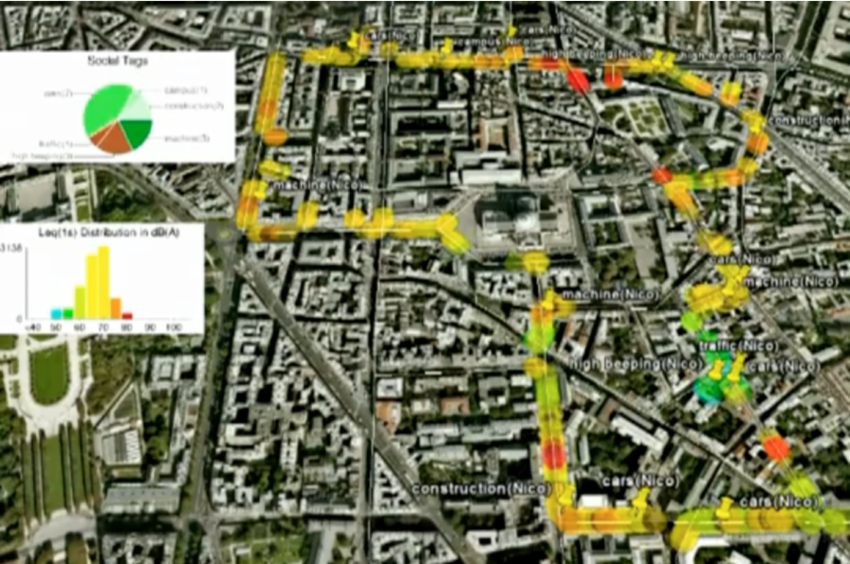
\includegraphics[scale=0.8]{app_noisetube.png}
    \fdireta{2010_Arnand}
\end{figure}

Outra área em que a vigilância participativa tem desempenhado um papel importante é a monitorização do ruído ambiental. O aplicativo NoiseTube permite que os usuários realizem medições de ruído e compartilhem esses dados, criando um mapa colaborativo do ruído em diferentes localidades. Essa vigilância participativa do ruído ambiental permite a identificação de áreas com altos níveis de ruído, auxiliando na tomada de medidas para mitigar os efeitos adversos na saúde e no bem-estar da comunidade. Ao participar ativamente da vigilância do ruído, os cidadãos contribuem para a criação de ambientes mais saudáveis e para a implementação de políticas públicas adequadas \cite{2010_Arnand}.

Esses exemplos ilustram como a vigilância participativa pode ser aplicada em diferentes áreas, além da saúde. Ao envolver os cidadãos na coleta e compartilhamento de informações relevantes, a vigilância participativa se torna uma ferramenta poderosa para a identificação e resposta a problemas ambientais e sociais. Essa abordagem colaborativa, combinada com o uso de tecnologias móveis e plataformas digitais, fortalece a relação entre a comunidade e as autoridades responsáveis, promovendo uma governança mais inclusiva e eficaz.

\subsection*{Iniciativa Brasil Sem Corona}

A Iniciativa Brasil Sem Corona, uma colaboração entre o Colab.re e a startup Epitrack, exemplifica o uso eficaz da tecnologia para facilitar a participação cidadã durante uma crise de saúde pública. Através desta iniciativa, os dados sobre a pandemia de COVID-19 foram coletados diretamente dos cidadãos, que relataram seus sintomas e receberam informações sobre como se proteger do vírus. Esses dados foram então utilizados para gerar mapas de calor que auxiliaram as autoridades de saúde a identificar e responder a surtos de COVID-19.

Na cidade de Caruaru/PE, a iniciativa teve resultados significativos. O projeto contou com 861 usuários ativos, apresentando uma média de 1,2 relatórios por usuário por semana. A plataforma Brasil Sem Corona começou em 20 de março e, desde então, tem sido oficialmente utilizada pela autoridade de saúde de Caruaru para melhorar a qualidade das informações do sistema de vigilância tradicional. Em relação aos casos de síndrome respiratória do sistema de vigilância tradicional, 1.588 indivíduos foram positivos para este resultado clínico. A análise de varredura espacial detectou 18 aglomerados e 6 deles apresentaram significância estatística (valor p < 0,1). Os aglomerados 3 e 4 apresentaram uma área de sobreposição que foi escolhida pela autoridade local para implantar a sorologia de Covid-19, onde 50 indivíduos foram testados. Desses, 32\% (n=16) apresentaram resultados reagentes para anticorpos relacionados à Covid-19 \cite[1]{2020_LealNeto}. Essa pesquisa demonstra como a vigilância participativa pode ser uma ferramenta eficaz para melhorar a qualidade das informações do sistema de vigilância tradicional, permitindo uma detecção precoce de surtos de COVID-19 e uma resposta mais eficaz, principalmente quando aliado a uma aplicação de alta disponibilidade e adoção pela população.

\section{Análise de Dados: Eventos e Distribuição Demográfica}

Com base nos dados disponibilizados pelo Colab.re para esse estudo, analisamos um total de 328.876 eventos criados entre 04/01/2013 e 05/12/2022. Para essa análise foi utilizado a linguagem Python e a biblioteca Pandas. O código fonte está disponível no GitHub.

\subsection*{Modelo de dados}

\begin{table}[ht]
	\centering
	\caption{Modelo de Dados da lista de usuários}
	\label{tab:user_model}
	\begin{tabularx}{\textwidth}{|l|X|}
		\hline
		\textbf{Campo}     & \textbf{Descrição}                              \\
		\hline
		colab\_user\_id    & Identificador único do usuário no sistema Colab \\
		gender             & Gênero do usuário                               \\
		birth\_date        & Data de nascimento do usuário                   \\
		city\_id           & Identificador único da cidade do usuário        \\
		city\_name         & Nome da cidade do usuário                       \\
		state\_id          & Identificador único do estado do usuário        \\
		state\_name        & Nome do estado do usuário                       \\
		created\_at        & Data de criação do registro do usuário          \\
		last\_sign\_in\_at & Data da última vez que o usuário fez login      \\
		device             & Dispositivo utilizado pelo usuário              \\
		\hline
	\end{tabularx}
\end{table}

\begin{table}[ht]
	\centering
	\caption{Modelo de Dados de eventos reportados}
	\label{tab:event_model}
	\begin{tabularx}{\textwidth}{|l|X|}
		\hline
		\textbf{Campo}    & \textbf{Descrição}                                   \\
		\hline
		event\_id         & Identificador único do evento                        \\
		user\_id          & Identificador único do usuário relacionado ao evento \\
		description       & Descrição do evento                                  \\
		status            & Status do evento                                     \\
		created\_at       & Data de criação do evento                            \\
		event\_type\_id   & Identificador único do tipo de evento                \\
		event\_type\_name & Nome do tipo de evento                               \\
		\hline
	\end{tabularx}
\end{table}

Os dados dos foram disponibilizados em formato CSV, contendo informações sobre os usuários e os eventos reportados. A \autoref{tab:user_model} apresenta o modelo de dados da lista de usuários. A \autoref{tab:event_model} apresenta o modelo de dados de eventos reportados.

\subsection*{Distribuição demográfica}

O quadro \autoref{quadro:usersbygender} apresenta a distribuição demográfica dos usuários por gênero. A maioria dos usuários se declararam do gênero másculino.


\begin{quadro}[htb]
	\caption{Usuários por gênero}
	\label{quadro:usersbygender}
	\centering
	\begin{tikzpicture}
		\pie[
			sum=auto,
			text=legend,
			radius=2
		]{
			60.10/Masculino,
			38.51/Feminino,
			0.03/Não Binário,
			1.36/Outro/Desconhecido
		}
	\end{tikzpicture}
	\begin{tabular}{|l|r|}
		\hline
		\textbf{Gênero} & \textbf{Quantidade} \\
		\hline
		Masculino       & 30494               \\
		Feminino        & 19555               \\
		Não Binário     & 16                  \\
		Desconhecido    & 335                 \\
		Outro           & 274                 \\
		Não Informado   & 92                  \\
		\hline
	\end{tabular}
\end{quadro}

\subsection*{Tipos de Eventos}

\begin{table}[h]
	\centering
	\caption{Tipos de eventos com mais ocorrências}
	\label{tab:tiposevento}
	\begin{tabularx}{\textwidth}{|X|l|l|}
		\hline
		\textbf{Tipo de Evento}                  & \textbf{Total de Ocorrências} \\
		\hline
		Entulho na calçada/via pública           & 61.785                        \\
		Buraco nas vias                          & 41.200                        \\
		Lâmpada apagada à noite                  & 32.907                        \\
		Ponto de infração de trânsito recorrente & 15.873                        \\
		Calçada irregular                        & 14.837                        \\
		Mato alto                                & 13.459                        \\
		Poda de árvore                           & 12.810                        \\
		Descarte irregular de lixo               & 12.685                        \\
		Bueiro entupido                          & 8.825                         \\
		Vazamento de água                        & 7.433                         \\
		Bueiro sem tampa                         & 5.844                         \\
		Ocupação irregular de área pública       & 5.714                         \\
		Fiação irregular                         & 5.643                         \\
		Veículo abandonado                       & 5.335                         \\
		Equipamento público danificado           & 4.694                         \\
		Esgoto a céu aberto                      & 4.656                         \\
		Retirada de árvore                       & 4.437                         \\
		Ponto recorrente de poluição sonora      & 4.189                         \\
		Bloqueio na via                          & 4.066                         \\
		Iluminação pública irregular             & 3.702                         \\
		\hline
	\end{tabularx}
\end{table}

A tabela \autoref{tab:tiposevento} apresenta os 20 tipos de evento mais reportados pelos usuários. A análise dos dados fornecidos pelos usuários do Colab proporcionou insights valiosos sobre as preocupações e demandas da comunidade. Os eventos mais frequentemente relatados estão intrinsecamente ligados a problemas e irregularidades na infraestrutura urbana, como entulho na calçada/via pública, buraco nas vias, lâmpada apagada à noite, ponto de infração de trânsito recorrente e calçada irregular. Essas ocorrências destacam a importância de investimentos contínuos na manutenção e melhoria da infraestrutura da cidade. Além disso, questões ambientais emergem como uma área de preocupação significativa, com denúncias frequentes de descarte irregular de lixo, desmatamento ilegal, esgoto a céu aberto e mato alto. Essas postagens indicam uma conscientização dos usuários em relação à preservação ambiental e ressaltam a necessidade de ações efetivas para aprimorar a gestão dos recursos naturais. O transporte público também é alvo de atenção, com reclamações recorrentes sobre problemas em ônibus, atrasos e superlotação. Esses aspectos exigem uma análise aprofundada das questões relacionadas à mobilidade urbana e podem impulsionar esforços para melhorar a qualidade e eficiência do transporte coletivo. Além disso, eventos relacionados à segurança e vigilância, como pontos de exploração sexual de menores e maus-tratos a animais, refletem a preocupação dos usuários com a proteção e bem-estar da comunidade. Por fim, a ocorrência de eventos envolvendo estabelecimentos comerciais, como falta de alvará e condições sanitárias irregulares, destaca a importância de ações rigorosas de fiscalização e de garantir a conformidade legal por parte dos estabelecimentos. Esses insights fornecem uma visão abrangente das preocupações dos usuários do Colab e podem orientar as prefeituras da cidade na implementação de políticas públicas que visem atender às demandas da comunidade e aprimorar a qualidade de vida em geral.

Os usuários estão engajados e ativos na identificação e denúncia de problemas na infraestrutura urbana, meio ambiente, transporte público e questões sociais. Isso indica uma participação cidadã ativa e um desejo de melhorar as condições de suas comunidades.
Os clientes podem aproveitar essas informações para acompanhar as preocupações e demandas da comunidade, tomar medidas corretivas mais efetivas e aprimorar a qualidade dos serviços e infraestrutura oferecidos.

Os dados fornecem uma visão clara das principais questões enfrentadas pela comunidade, permitindo que as prefeituras priorizem recursos e esforços em áreas críticas, como manutenção da infraestrutura, gestão ambiental, transporte público e segurança. As prefeituras podem usar esses insights para desenvolver políticas públicas mais eficazes, implementar medidas preventivas e corretivas, bem como estabelecer canais de comunicação e interação mais robustos com os cidadãos, fortalecendo a confiança e a participação da comunidade nas decisões governamentais.

\subsection*{Frequência de postagens e engajamento}

\begin{quadro}[htb]
	\caption{Histograma demonstrando a distribuição de novos eventos por ano}
	\label{quadro:colab_events_overtime}
	\centering
	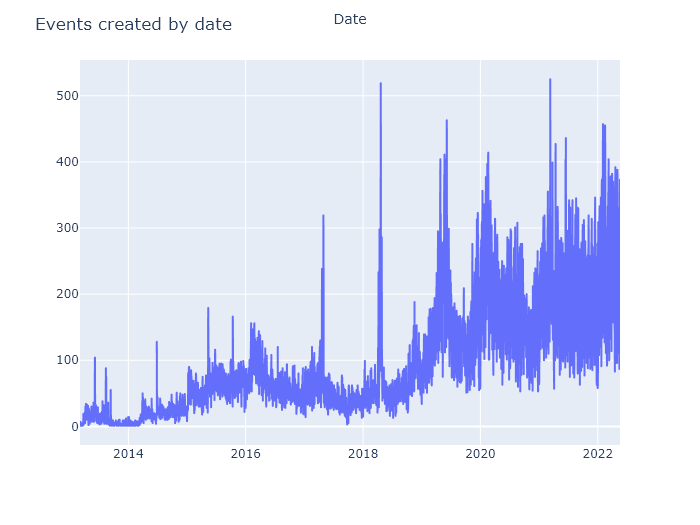
\includegraphics[scale=0.5]{colab_events_overtime.png}
\end{quadro}

O \autoref{quadro:colab_events_overtime} demonstra a criação de eventos ao longo dos anos. Na imagem pode-se identificar dois picos de mais de 500 postagens por mês: Abril de 2018 e Março de 2022. O primeiro pico, em abril de 2018, com 513 postagens, pode ser atribuído a []. Já o segundo pico, em março de 2022, com 528 postagens, pode ser explicado pela pandemia de COVID-19, que fez com que as pessoas passassem mais tempo em casa e, consequentemente, observassem mais problemas na infraestrutura urbana.

Além desses picos, é possível observar uma tendência geral de crescimento no número de postagens ao longo dos anos, com algumas flutuações. Por exemplo, em 2017, o número médio de postagens por mês foi de 231, enquanto em 2022, esse número aumentou para uma média de 389 postagens por mês. Isso sugere um aumento no engajamento dos usuários com o aplicativo Colab.re ao longo do tempo.

Também é interessante notar que o número de postagens tende a aumentar no início do ano, com picos observados em março de cada ano. Isso pode ser devido a fatores sazonais, como o aumento das chuvas no início do ano, que podem levar a mais problemas de infraestrutura urbana sendo relatados.

\section{Insights sobre o Colab.re}
As soluções de empresas Gov Tech tem se mostrado uma abordagem promissora para fortalecer a relação entre os cidadãos e os órgãos governamentais, proporcionando uma maior participação e engajamento da sociedade na tomada de decisões e na resolução de problemas em suas comunidades. Neste capítulo, exploramos o papel das plataformas digitais como ferramentas para promover a governança participativa, analisando um estudo de caso de uma plataforma de engajamento cívico.

Ao longo da discussão, destacamos a importância da inclusão digital como um fator fundamental para garantir o acesso equitativo às plataformas de participação. É essencial que os governos se empenhem em fornecer recursos e infraestrutura adequada, além de promover programas de capacitação digital, a fim de superar as barreiras existentes e permitir que todos os cidadãos tenham a oportunidade de participar ativamente.

Um dos principais benefícios observados é a ampliação do alcance e da diversidade das vozes representadas. A plataforma de engajamento cívico analisada atraiu um número significativo de usuários, dos quais foi possível extrair valiosos insights sobre as necessidades, preocupações e preferências da comunidade. Através da análise dos perfis dos usuários e das postagens, foi possível identificar tendências, prioridades e problemas recorrentes, fornecendo subsídios importantes para a formulação de políticas públicas mais eficazes e direcionadas.

A análise dos dados revelou que a plataforma atraiu uma participação equilibrada entre os gêneros, com uma representatividade significativa de usuários do gênero masculino e feminino. Além disso, também foi identificada a presença de usuários não binários e outros/desconhecidos, indicando uma diversidade de gênero na participação cívica. Esse aspecto é fundamental para garantir uma governança inclusiva e representativa, onde todas as vozes sejam ouvidas e consideradas na tomada de decisões.

Entre os principais tipos de eventos relatados pelos usuários na plataforma, destacaram-se problemas relacionados a entulho na calçada/via pública, buracos nas vias, lâmpadas apagadas à noite e pontos de infração de trânsito recorrentes. Esses dados fornecem um panorama dos principais desafios enfrentados pela comunidade, permitindo que os órgãos governamentais priorizem ações e aloquem recursos de forma mais eficiente, direcionando esforços para áreas que necessitam de intervenção imediata.

No entanto, é importante ressaltar que as plataformas de engajamento cívico são apenas uma parte do processo de governança participativa. Elas devem ser complementadas por outros mecanismos de participação, como audiências públicas, consultas presenciais e parcerias com organizações da sociedade civil. A combinação dessas abordagens pode gerar resultados mais abrangentes e inclusivos, evitando a exclusão digital e garantindo a participação de todos os segmentos da sociedade.

Além disso, é fundamental que as plataformas sejam projetadas levando em consideração a usabilidade, a acessibilidade e a segurança dos dados dos usuários. Políticas claras de privacidade e proteção de dados devem ser implementadas, garantindo a confidencialidade das informações compartilhadas e a confiança dos usuários na plataforma.

No contexto em constante evolução das tecnologias digitais, é importante que os governos e as comunidades estejam abertos a inovações e melhorias contínuas nas plataformas de engajamento cívico. A coleta e análise de dados podem fornecer insights valiosos sobre as demandas e expectativas da comunidade, permitindo a adaptação e o aprimoramento das estratégias de participação.

Em suma, a governança participativa mediada por plataformas digitais oferece oportunidades únicas para envolver os cidadãos no processo decisório, promover a transparência e a prestação de contas, e direcionar recursos de forma mais eficiente. No entanto, é essencial que essas plataformas sejam implementadas de forma inclusiva, acessível e segura, garantindo a representatividade e a diversidade das vozes participantes. Ao explorar o potencial das plataformas de engajamento cívico, os governos podem fortalecer a democracia e criar comunidades mais participativas e resilientes.